\section{Multi-precision calculations}

Using Jacobi polynomials as bases functions have the potential problem of inducing considerable precision loss in the calculations.
From the symbolic expressions to the end results, there are multiple stages that are prone to such precision loss:
\begin{enumerate}
    \item Calculation of Gauss-Jacobi nodes and weights. This is especially problematic when high degrees or unbalanced ($\alpha$, $\beta$) indices are used. The former stacks the nodes increasingly densely at the boundaries, and the latter pushes the Jacobi polynomials to be skewed towards one side, worsening the phenomenon.
    \item Numerical quadrature. Using Jacobi polynomials and their derivatives is prone to considerable precision loss during quadrature, as the amplitude is unbalanced (not equiripple?). The fact is also noticed by the Dedalus team in \href{https://github.com/DedalusProject/dedalus/issues/166}{this issue}. The extent of precision loss of course depends on the actual truncation degree used. For $N=50$, a precision loss of 5 orders of magnitude or more has been experienced (i.e. an element that should be zero in the mass matrix can be $\sim 10^{-10}$ when using the correct Gauss-Jacobi quadrature to double precision).
    \item Eigenvalue problem solver. This will probably not be a major issue (the precision loss is expected to be lower than that in quadrature). However, if solutions of higher precision is sought, the eigensolver naturally needs to work under at least the desired output precision, if not higher.
\end{enumerate}

There are three python packages that are capable of handling multi-precision calculations:
\begin{itemize}
    \item The \textbf{Sym}bolic \textbf{Py}thon library \colorbox{backcolour}{\lstinline|sympy|}. This is also the package on which the symbolic part of \colorbox{backcolour}{\lstinline|plesiogeostropy|} is implemented. The evaluation can be to arbitrary precision, similar to the design concept in \texttt{Mathematica}. However, \colorbox{backcolour}{\lstinline|sympy|} is mostly a symbolic package. Its multi-precision calculation is not at all efficient, and will not be a good candidate for multi-precision linear algebra.
    %
    \item The \textbf{M}ulti-\textbf{P}recision \textbf{Math} library \colorbox{backcolour}{\lstinline|mpmath|}. This is the go-to library for general-purpose multi-precision calculations. It has a rich library of functions that support multi-precision computations.
    %
    \item The \textbf{G}NU \textbf{M}ulti-\textbf{P}recision \textbf{Py}thon extension module \colorbox{backcolour}{\lstinline|gmpy2|}. This is a C-coded Python extension library. It offers a less comprehensive library for general-purpose calculations, but is several times faster than \colorbox{backcolour}{\lstinline|mpmath|} on basic arithmetics, thus has an edge when it comes to large linear algebra problems.
\end{itemize}

\noindent \todoitem{Multi-precision Gauss-Jacobi nodes and weights}

\noindent \todoitem{Different multi-precision library; using multi-precision data types in numpy arrays}

\noindent \todoitem{Multi-precision linear algebra: flamp}

The "sparsity" of the matrices show that the current multiple precision implementation removes the obstacle posed by precision loss in quadrature.

\begin{figure}[htbp]
    \centering
    \includegraphics[width=\linewidth]{../../out/eigen/Malkus/Reduced/matview_prec-np.png}
    \caption{Logarithmic absolute values of matrix elements ($\log(A_{ij})$) for the Malkus background field eigenproblem, calculated using numpy/scipy to double-precision.}
\end{figure}

\begin{figure}[htbp]
    \centering
    \includegraphics[width=\linewidth]{../../out/eigen/Malkus/Reduced/matview_prec-113.png}
    \caption{Logarithmic absolute values of matrix elements ($\log(A_{ij})$) for the Malkus background field eigenproblem, calculated using gmpy2 to 113 bits precision (equiv. quadrupole precision).}
\end{figure}

The final results for the Malkus field also show that the multi-precision implementation is able to obtain solutions that are accurate to much higher precision.
The error is at the level of quadrupole precision for low order modes.
However, we do see a considerable increase in error for the overtones, the cause of which is unclear. Possible candidate is the eigensolver. Nevertheless, the level of error is unlikely to be relevant for obtaining results that are accurate to double precision.

\begin{figure}[htbp]
    \centering
    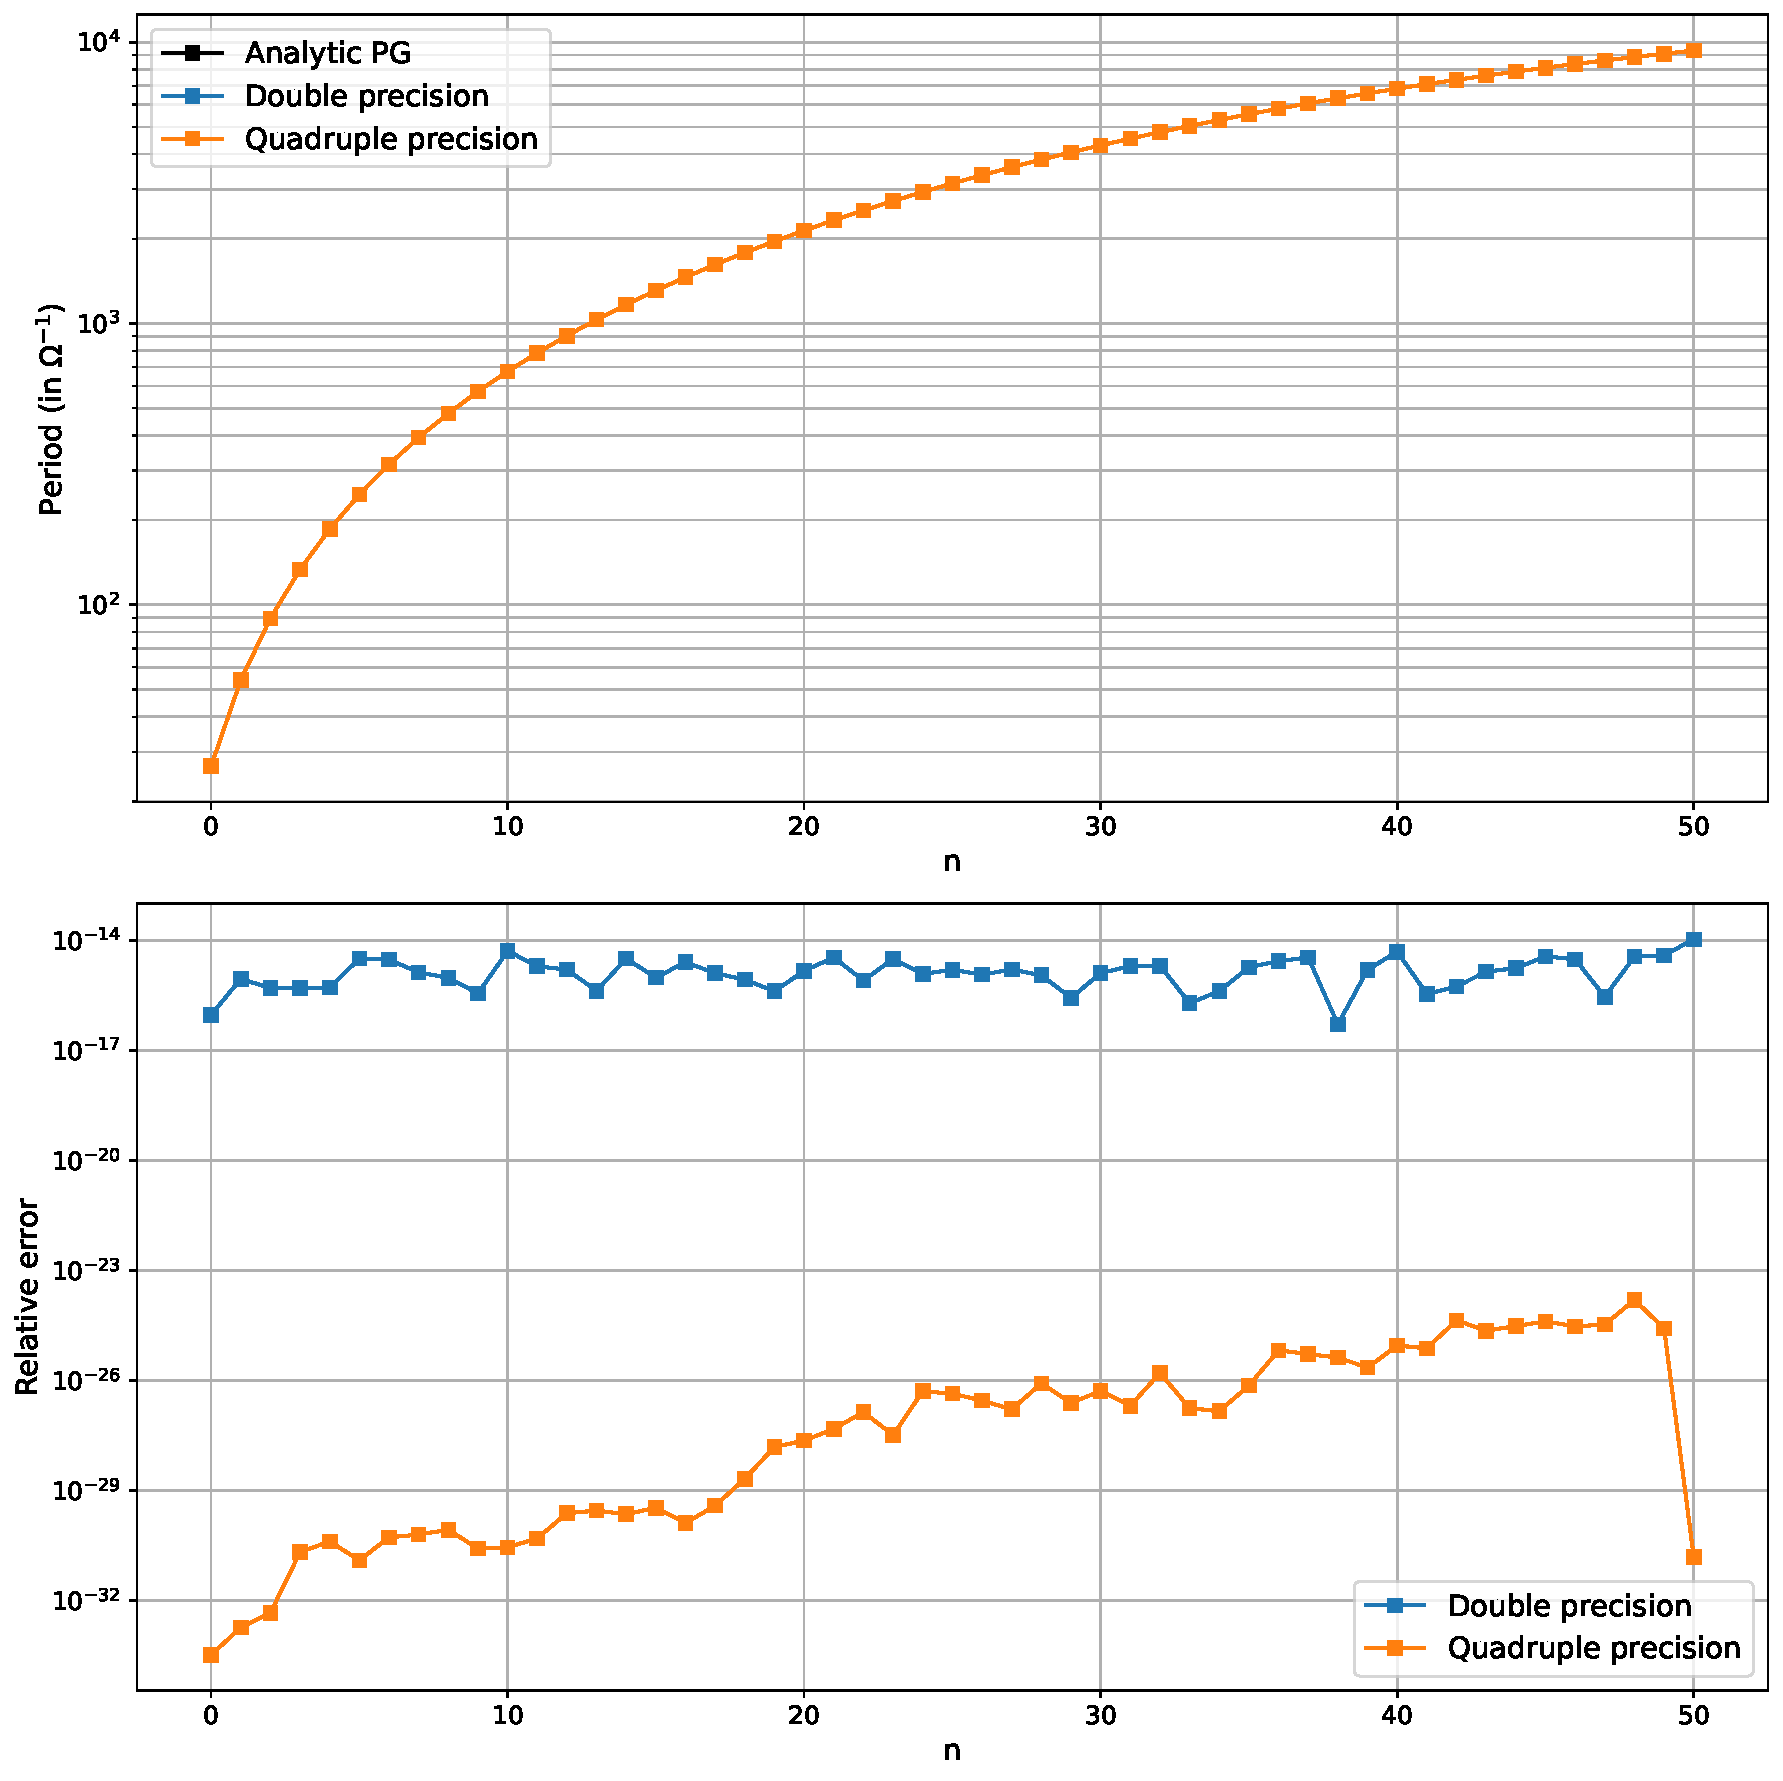
\includegraphics[width=.8\linewidth]{../../out/eigen/Malkus/Reduced/Analytical_error_precision_fast.pdf}
    \caption{Eigenperiods (upper panel) for $m=3$ fast modes under Malkus background field, solved to double precision and quadruple precision, with their respective errors from the analytical solution (lower panel). Both calculations are done using the reduced system and a truncation level $N=50$.}
\end{figure}

\begin{figure}[htbp]
    \centering
    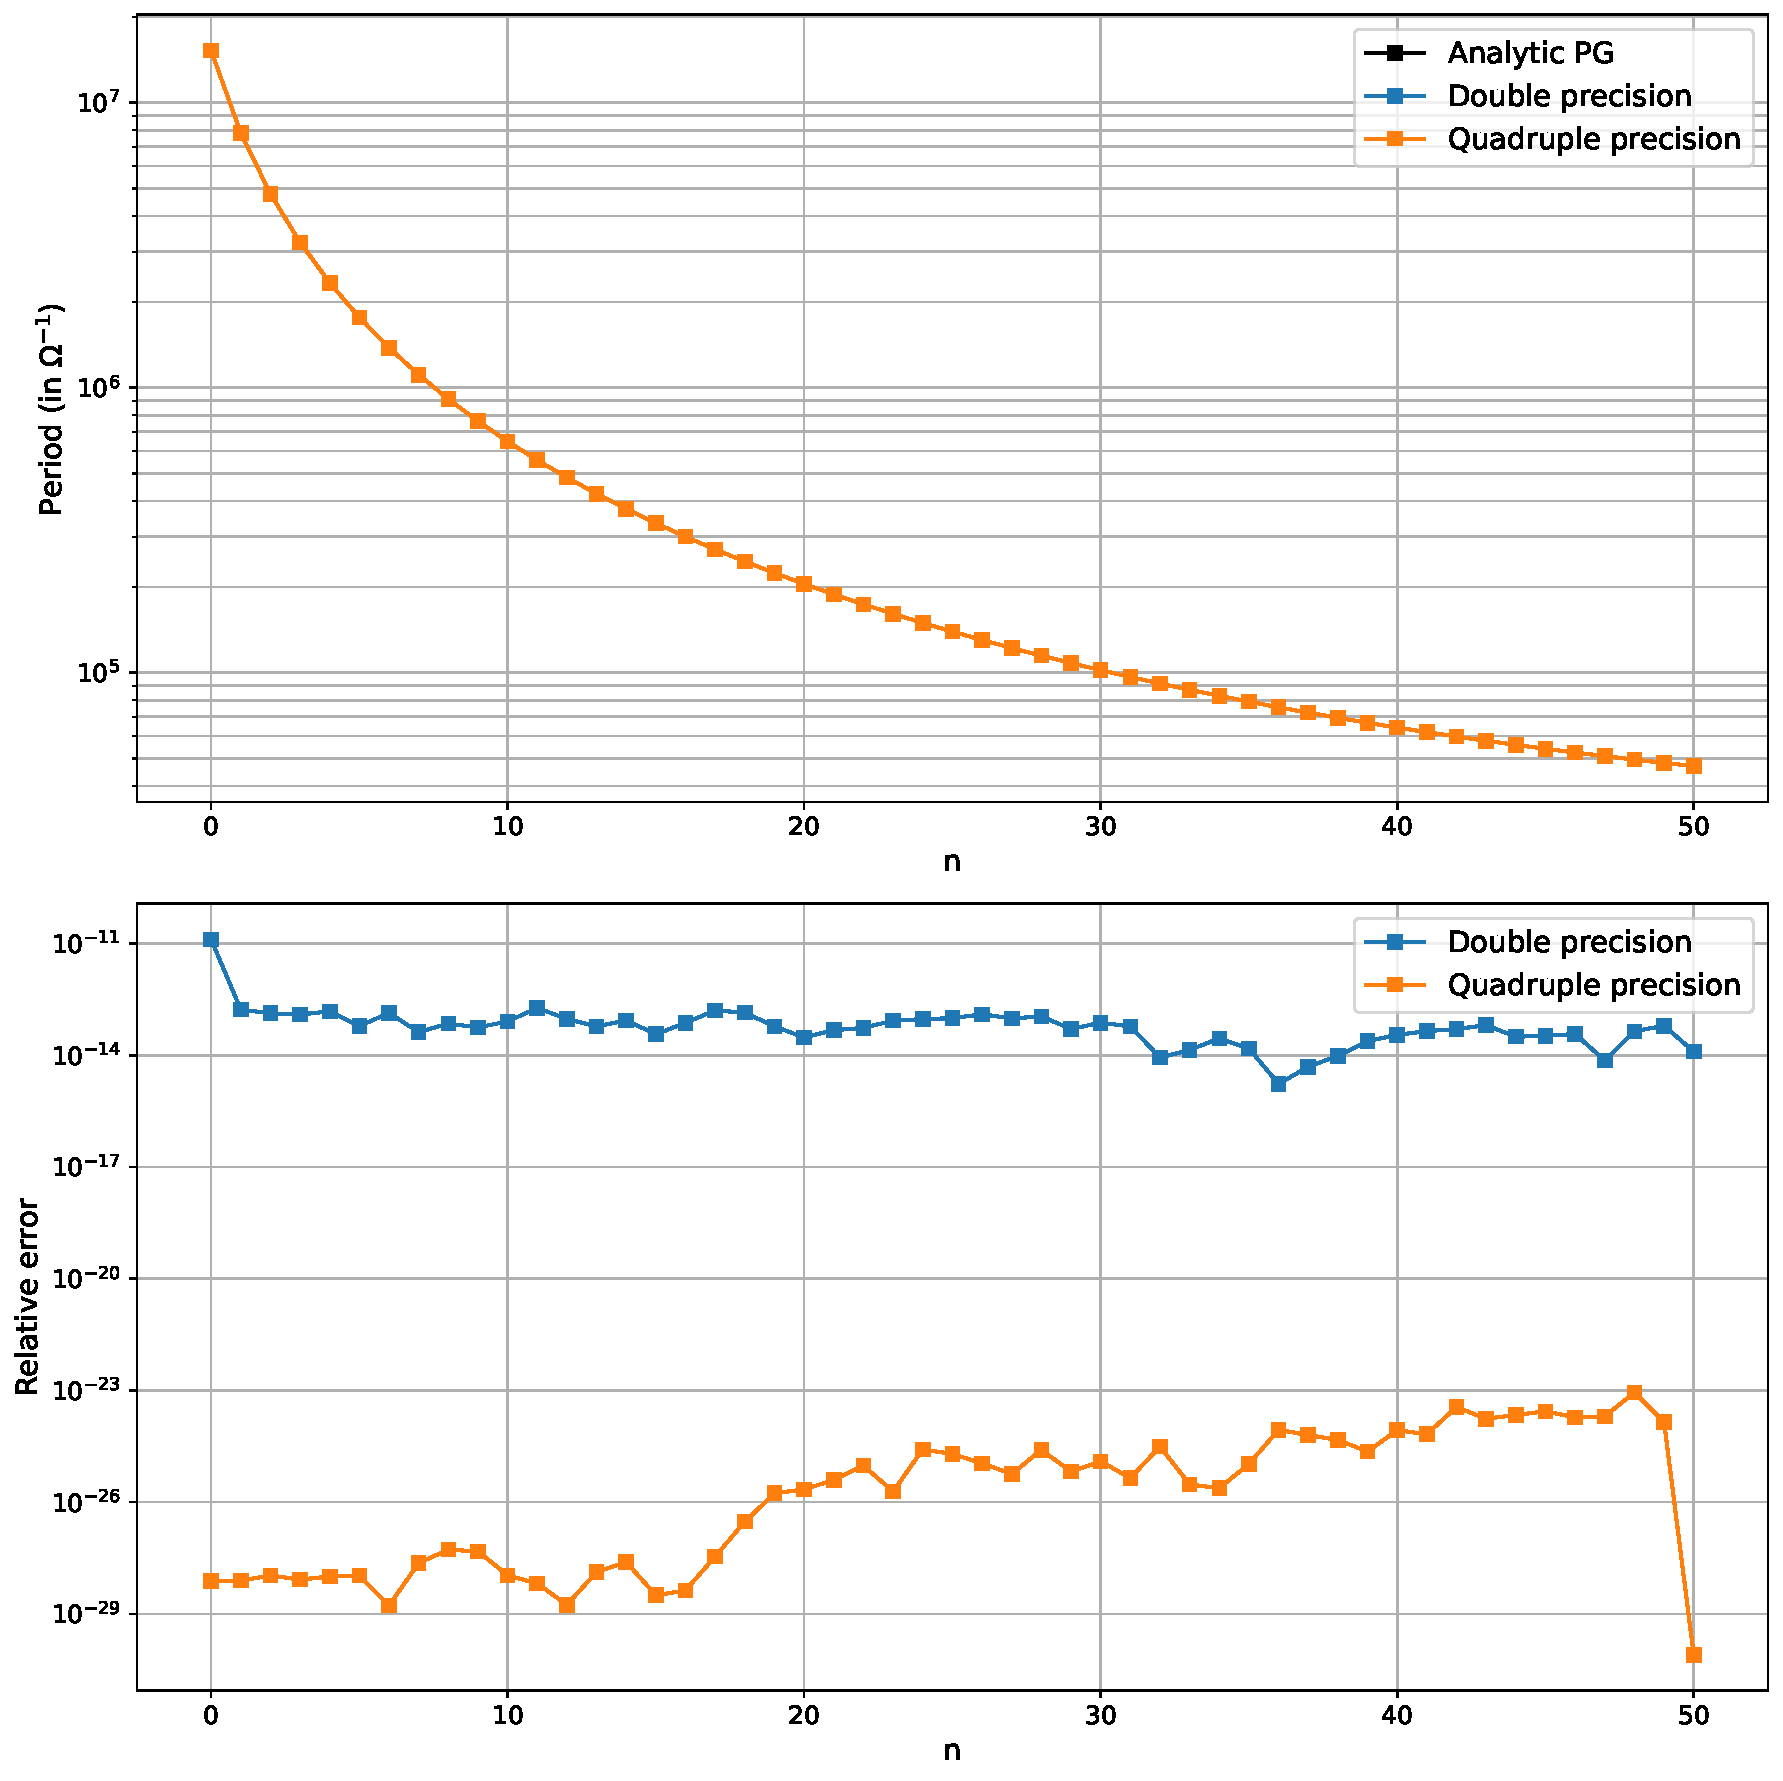
\includegraphics[width=.8\linewidth]{../../out/eigen/Malkus/Reduced/Analytical_error_precision_slow.pdf}
    \caption{Eigenperiods (upper panel) for $m=3$ slow modes under Malkus background field, solved to double precision and quadruple precision, with their respective errors from the analytical solution (lower panel). Both calculations are done using the reduced system and a truncation level $N=50$.}
\end{figure}

